\section{Navigazione e contenuto testuale}\label{contenav}

La navigazione all'interno del sito è resa molto facile in quanto TicketOne è principalmente composto da pagine di eventi.

\subsection{Navigazione}
	TicketOne non implementa nessuna particolare regola nel dire all'utente la pagina in cui si trova.
	Come per gli eventi, ciascuna pagina ha il nome dell'evento o della categoria a cui appartiene sotto allo slogan, in alto a sinistra.
	L'assenza di \textit{breadcrumb} non aiuta molto l'utente, anzi potrebbe confonderlo se entra dal sito in una pagina secondaria tramite un motore di ricerca e non arrivandoci dall'homepage.
	\par Cliccando sul logo di TicketOne è possibile tornare all'homepage e da lì spostarsi nelle altre parti del sito tramite la ricerca o utilizzando la suddivisione degli eventi in categorie.

\subsection{Footer}
	Come per altri siti e piattaforme, il \textit{footer} di TicketOne contiene informazioni utili per l'utente come: collegamenti alle pagine statiche informative, ulteriori servizi secondari, collegamenti ai social, collegamento alla pagina delle domande frequenti, informazioni su come contattare il call center, ecc.

	\begin{figure}[hbt]
		\centering
		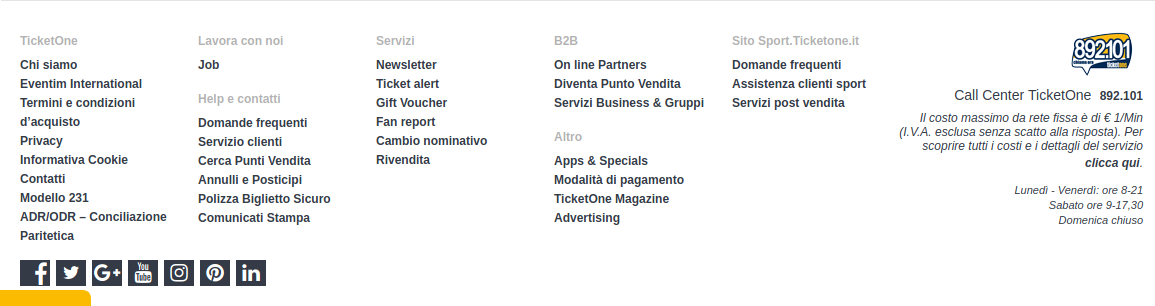
\includegraphics[width=\textwidth]{img/footer.png}
		\caption{Footer TicketOne}
		\label{footer}
	\end{figure}

	Questa parte dell'interfaccia rimane statica e si ripete nella stessa maniera in ogni pagina.
	\par Il footer, nonostante sia la parte meno visitata dagli utenti, resta molto importante in quanto contiene collegamenti utili per la navigazione del sito.

\subsection{Paragrafi}
	In tutto il sito i paragrafi sono corti e ciascun con un proprio titolo.
	Questa separazione visiva permette all'utente una lettura più scorrevole evitando l'eccesso di testo che potrebbe aggiungere informazioni inutili e fare che l'utente vada via.
	\par Vi sono tuttavia certi paragrafi che possono avere un maggior contenuto testuale, come per esempio gli avvisi posti prima della lista dei biglietti disponibili (Fig.~\ref{when}).
	Questi tuttavia possono essere giustificati in quanto il testo contiene informazioni importanti relative all'evento in questione.
	\par Altre parti del sito, come ad esempio le pagine statiche, contengono testo scritto in maniera molto discorsiva, come ad esempio le pagine in cui vi sono le informazioni legali.
